\chapter{Glance Configuration}
%Intro\footnotemark\\
\begin{spacing}{1.2}
%note en bas de page


\par The Image service (glance) project provides a service in which users can download
and discover data assets for use with other services. This includes
currently images and metadata definitions. \\

\section{Add users and others for Glance in Keystone.}

\par To start, we will create a user [glance] in the project [service]. 
Then We will add this user [glance] in the role [admin] and create a service entry
for [glance]:  \\
\\
\begin{figure}[!htb] 
\begin{center} 
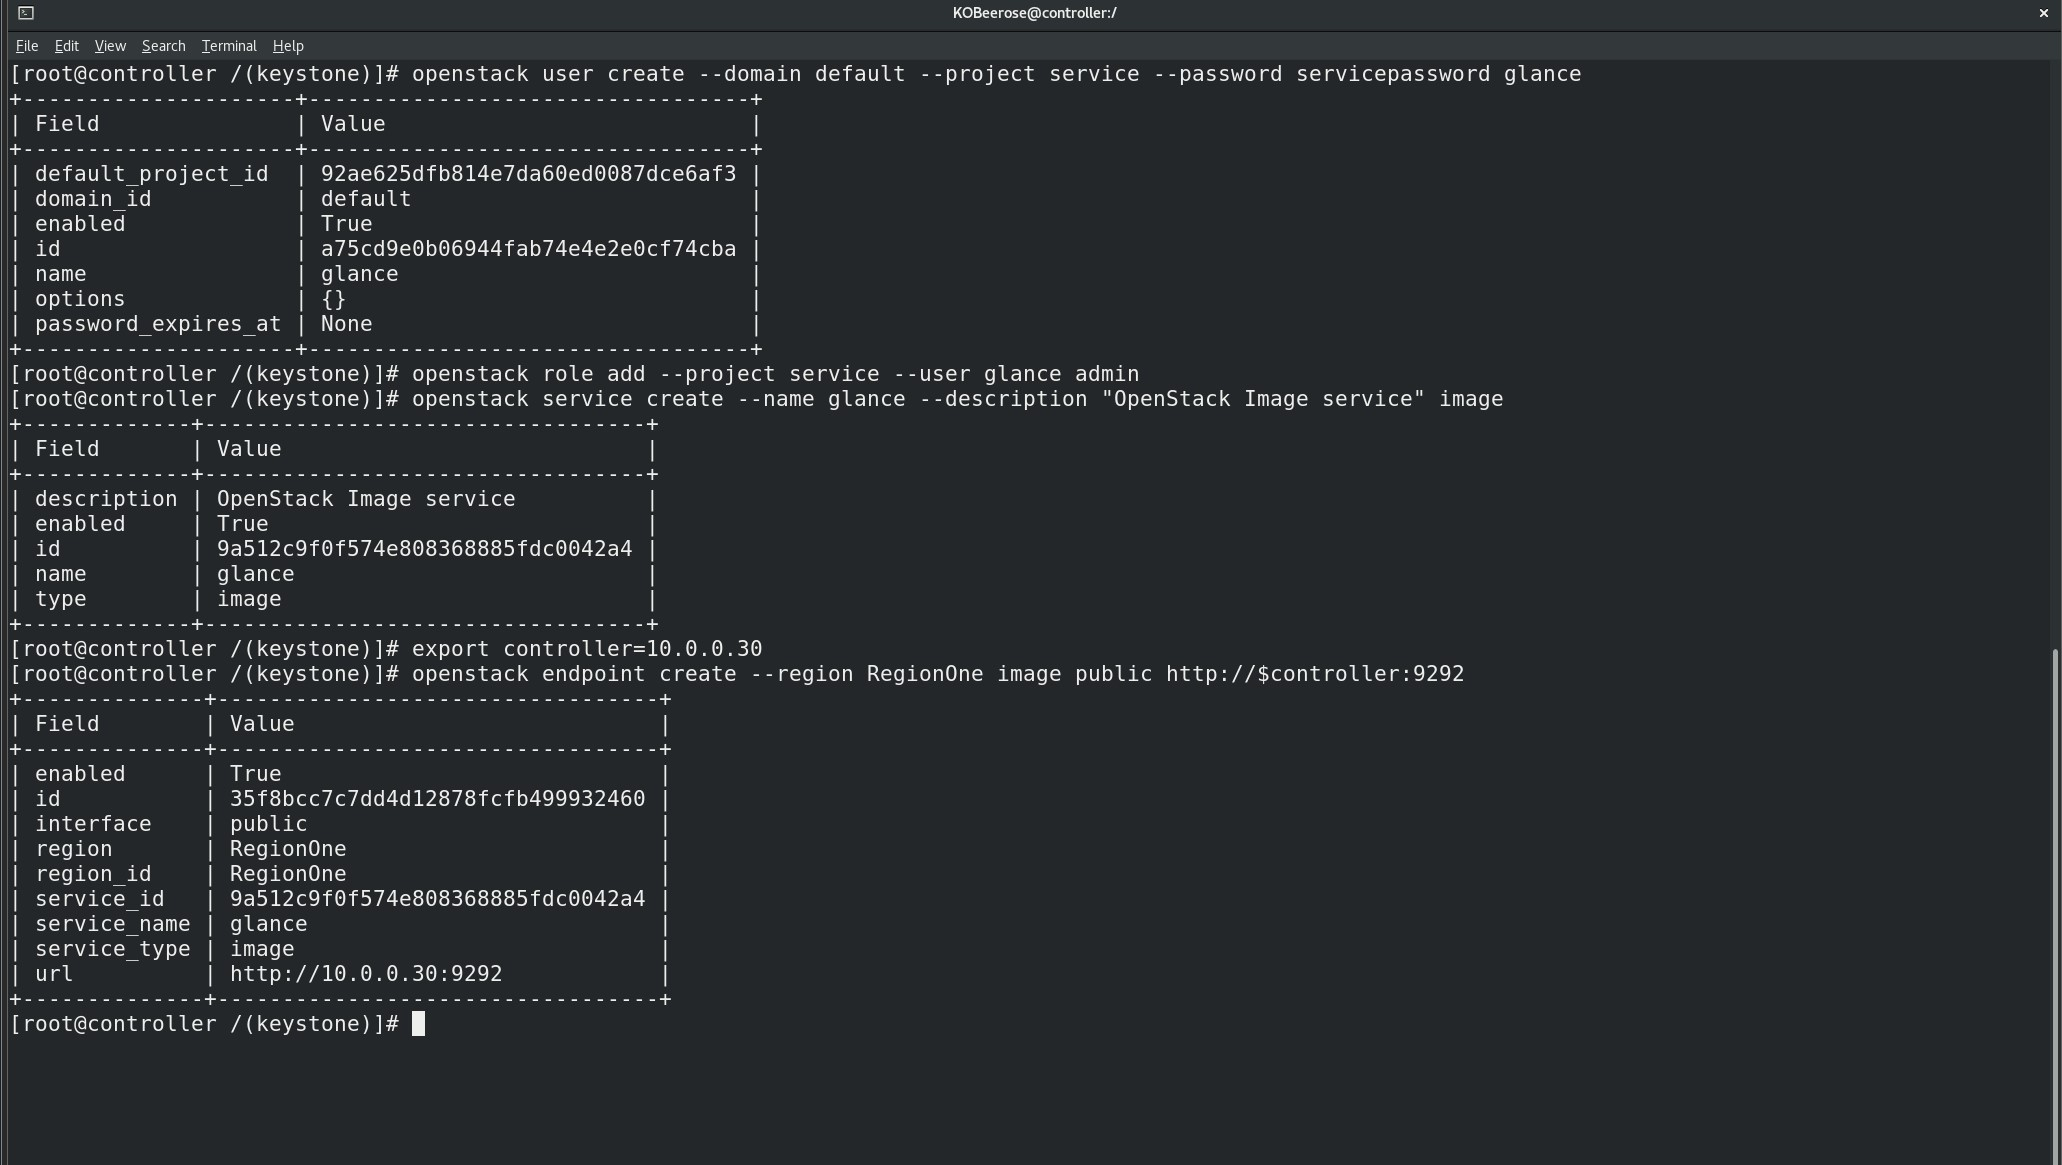
\includegraphics[width=1\linewidth]{Cloud/Configure Glance/Adding users for glance} 
\end{center} 
\caption{Adding users for glance} 
\end{figure}  \FloatBarrier
\\


\par Next, we'll define the Glance API host by exporting the controller, then we'll create an Endpoint for [glance] (public, internal and administrator): 
\\
\begin{figure}[!htb] 
\begin{center} 
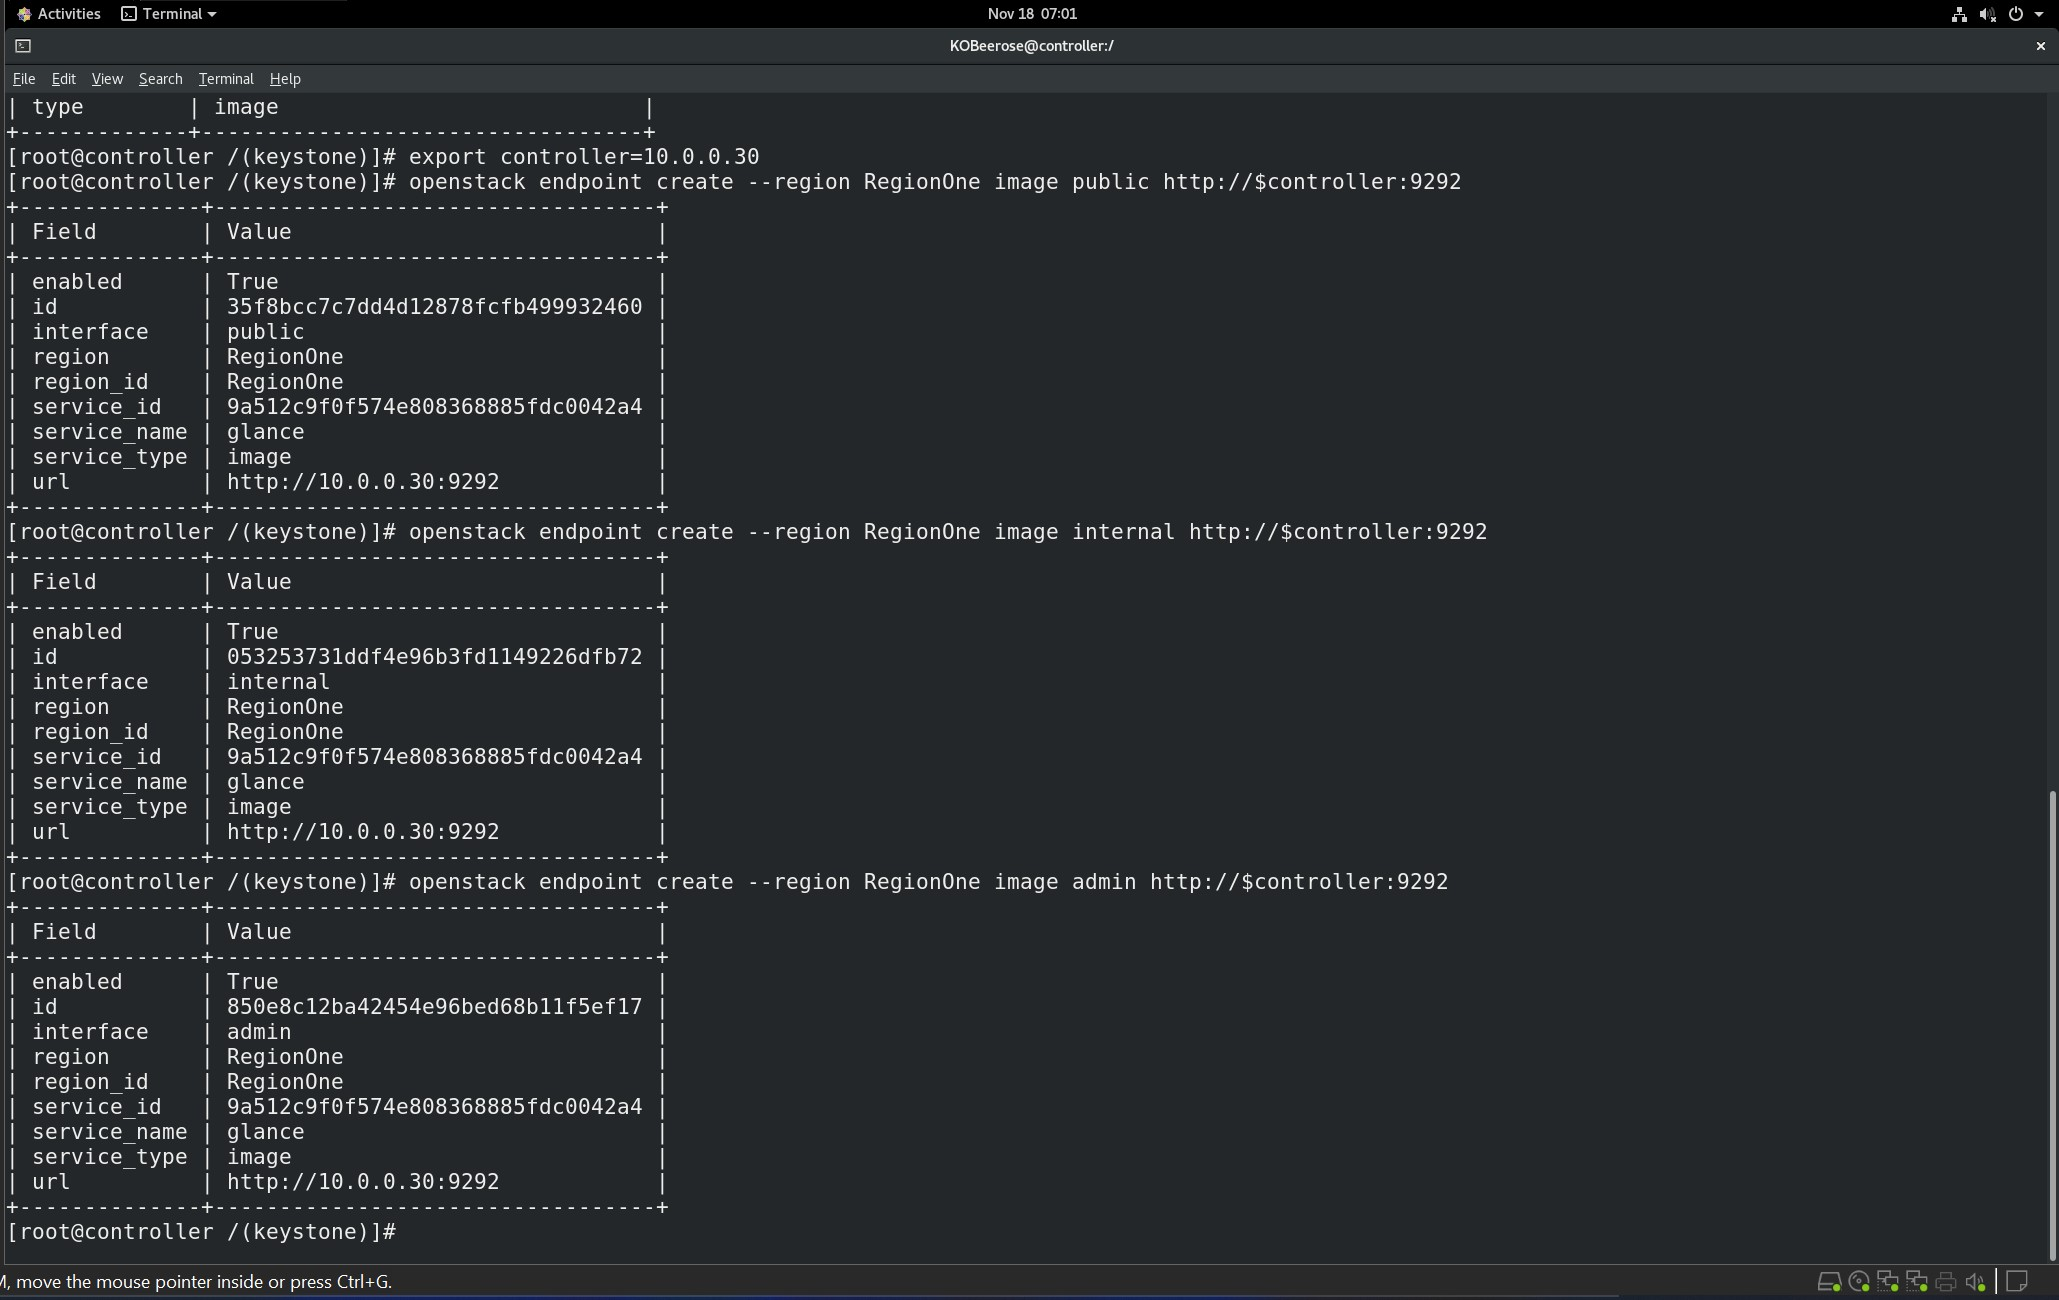
\includegraphics[width=1\linewidth]{Cloud/Configure Glance/Creating Endpoints for glance} 
\end{center} 
\caption{Creating Endpoints for glance} 
\end{figure}  \FloatBarrier
\\



\section{Adding a User and Database on MariaDB for Glance.}

\par As we did for Keystone, we will also add a user and a database on MariaDB for Glance.\\

\\
\begin{figure}[!htb] 
\begin{center} 
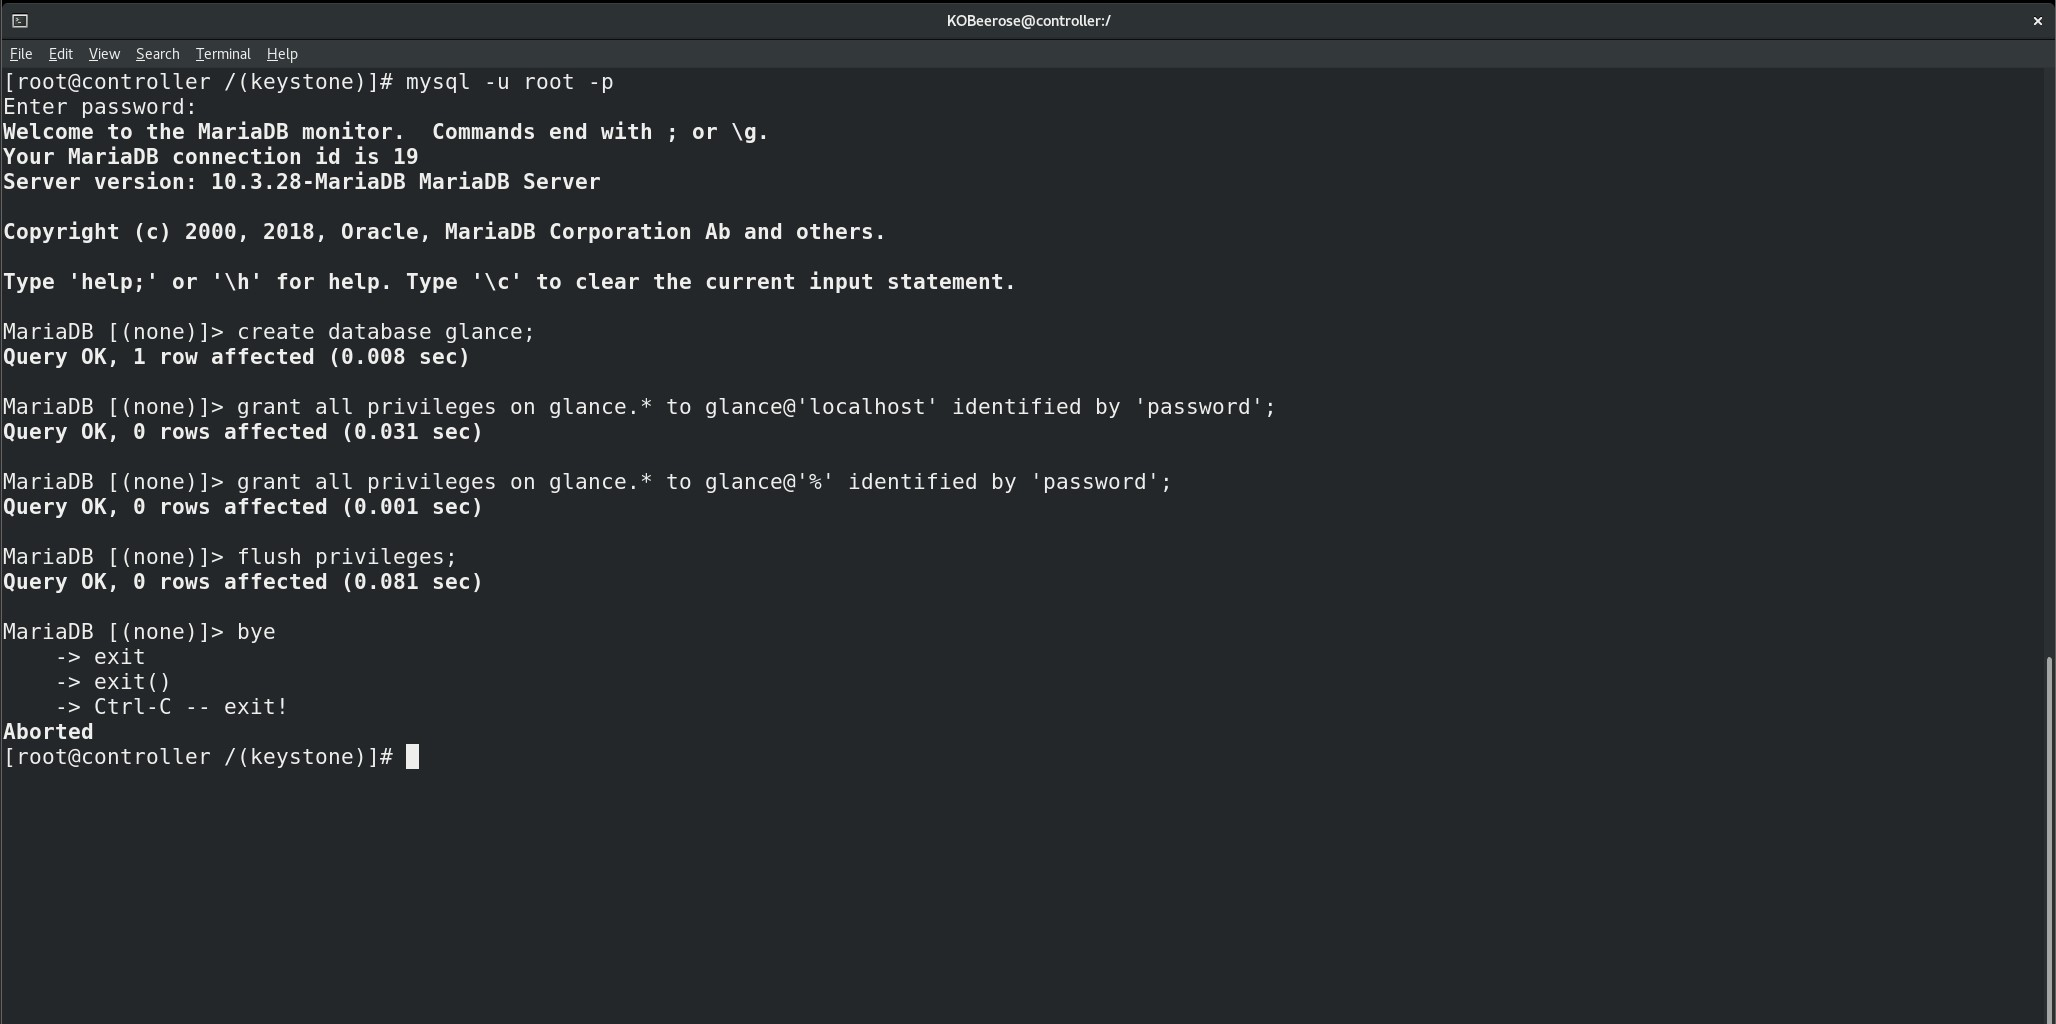
\includegraphics[width=1\linewidth]{Cloud/Configure Glance/Add a user and DB for glance} 
\end{center} 
\caption{Add a user and DB for glance} 
\end{figure}  \FloatBarrier
\\

\section{Installation and Configuration of Glance.}
\par We will check that openstack-glance is installed, to start the glance api configuration, for that we will create a new file /etc/glance/glance-api.conf as shown below below to add MariaDB login information and authentication information
keystone, and after that we will enable openstack-glance-api. 
\\
\begin{figure}[!htb] 
\begin{center} 
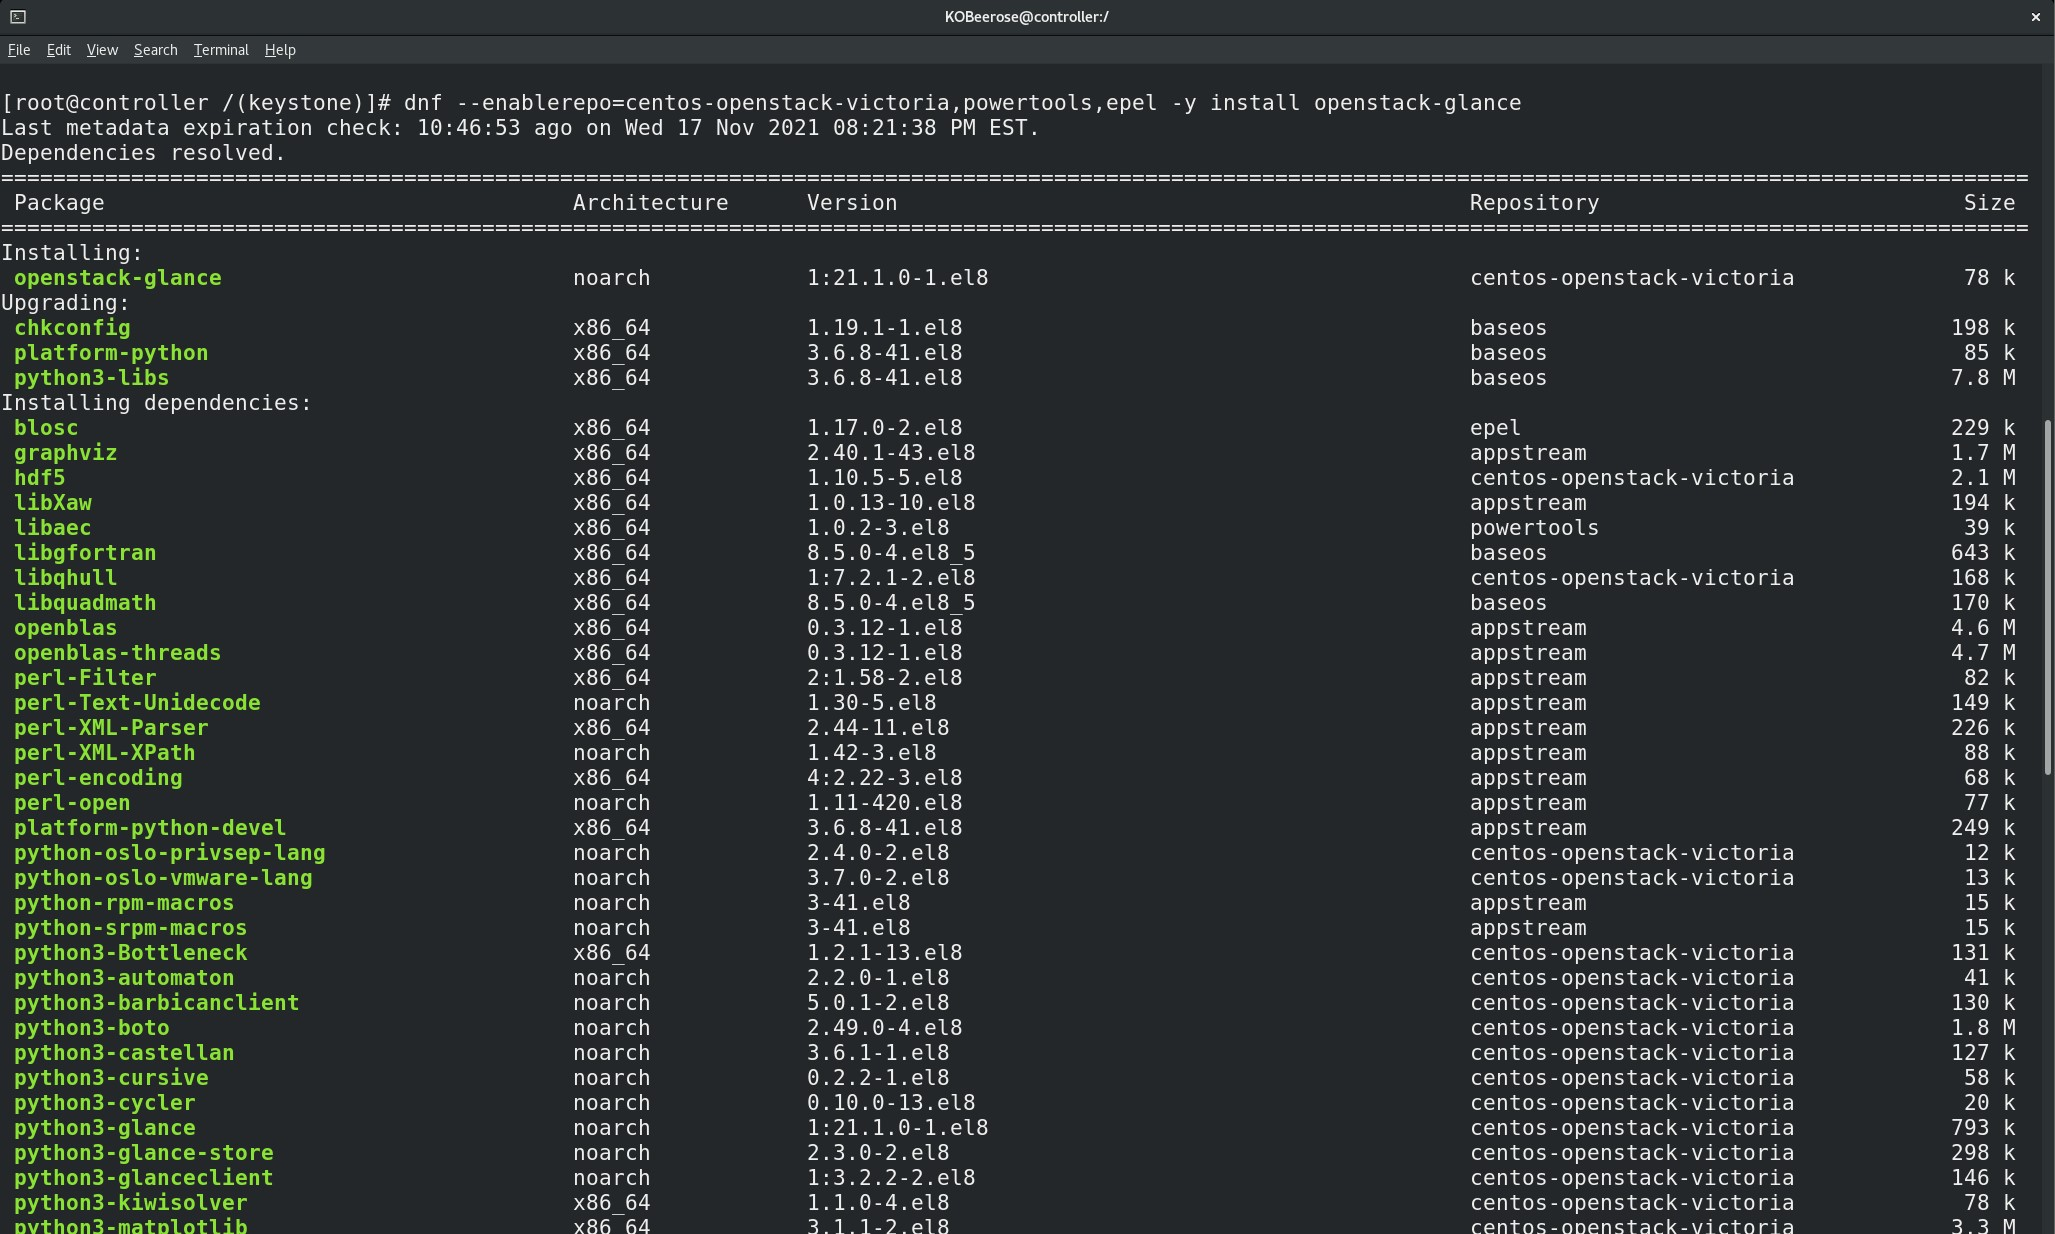
\includegraphics[width=1\linewidth]{Cloud/Configure Glance/Installing Glance} 
\end{center} 
\caption{Installing Glance} 
\end{figure}  \FloatBarrier
\\
\\
\begin{figure}[!htb] 
\begin{center} 
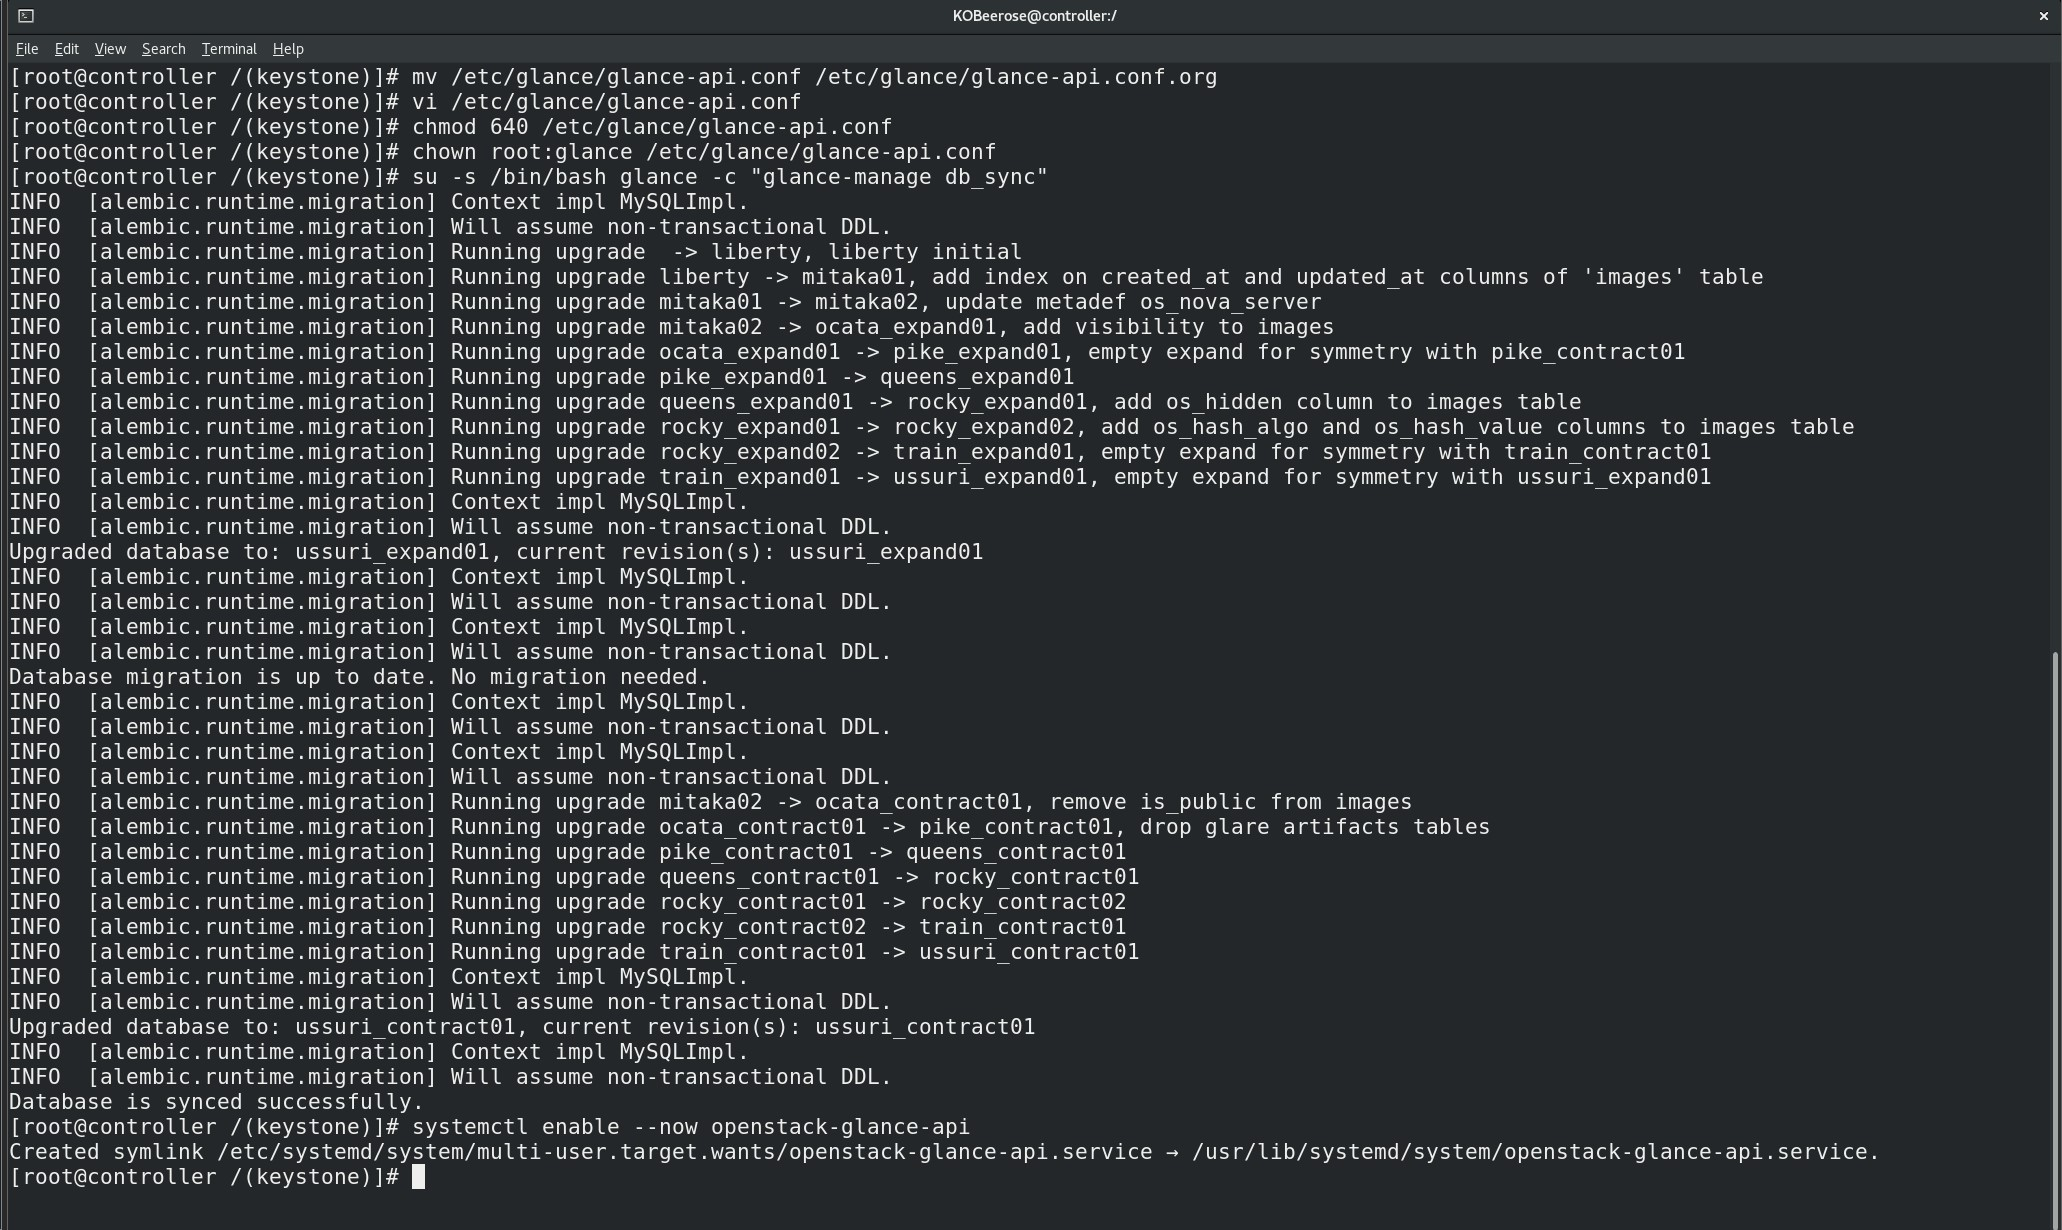
\includegraphics[width=1\linewidth]{Cloud/Configure Glance/Configuring Glance} 
\end{center} 
\caption{Configuring Glance} 
\end{figure}  \FloatBarrier
\\


\section{glanceapi.te config}
\par 
Finally we will modify some boolean seLinux parameters about glance api can network, we will create the policy file glanceapi.te to compile it. 
\\
\begin{figure}[!htb] 
\begin{center} 
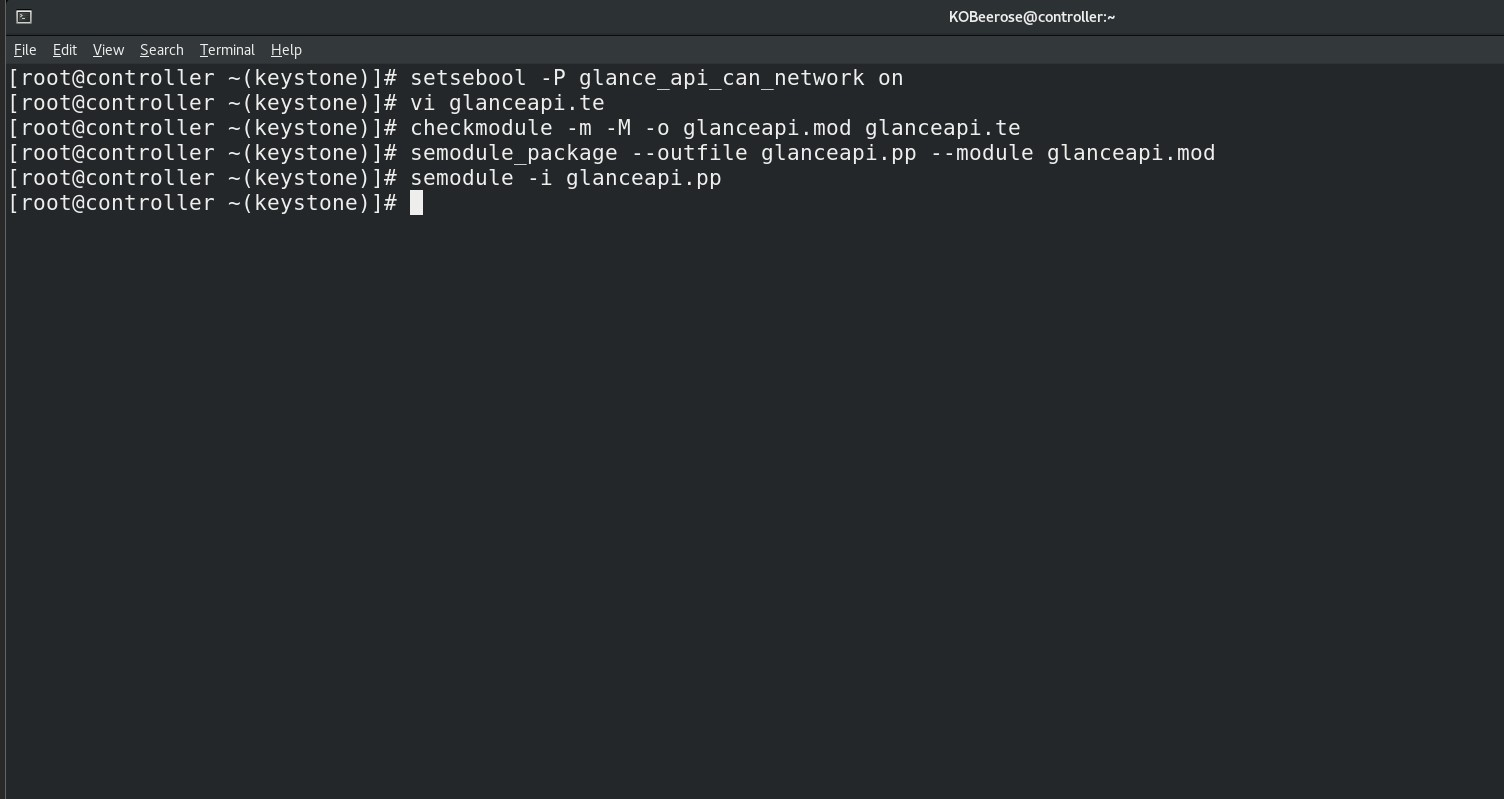
\includegraphics[width=1\linewidth]{Cloud/Configure Glance/Config for glanceapi} 
\end{center} 
\caption{Config for glanceapi} 
\end{figure}  \FloatBarrier
\\

\par 
Now we are going to allow the port 9292 service and reloading the firewall.
\\
\begin{figure}[!htb] 
\begin{center} 
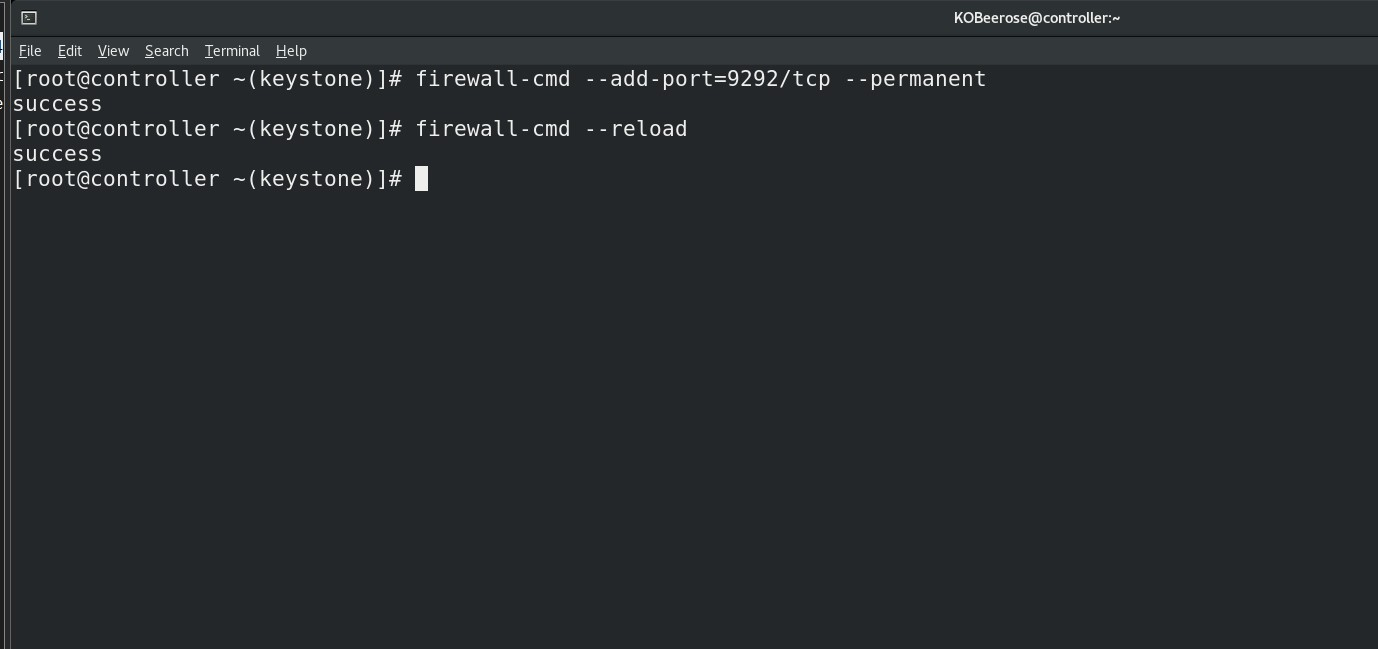
\includegraphics[width=1\linewidth]{Cloud/Configure Glance/Allowing 9292 port.} 
\end{center} 
\caption{Allowing 9292 port.} 
\end{figure}  \FloatBarrier
\\


\end{spacing}